\begin{anexosenv}

\partanexos

\chapter{Primeiro Anexo}

Texto do primeiro anexo.

\chapter{Metodologia IPHAN de Gestão de Demandas de Desenvolvimento Ágil de Software}

O MIDAS foi baseado nos príncipios ágeis advindos do Manifesto Ágil, tais princípios foram adaptados ao contexto do órgão. Os princípios norteadores deste modelo foram:
\begin{itemize}
\item Envolvimento do requisitante (cliente): as áreas requisitantes estarão profundamente envolvidas no processo de desenvolvimento. Seu papel será fornecer e priorizar novos requisitos dos sistemas e avaliar as iterações.
\item Entrega incremental: o software é desenvolvido em incrementos e o cliente especifica os requisitos a serem incluídos em cada incremento.
\item Foco nos resultados e não no processo: a equipe de desenvolvimento deve desenvolver suas próprias maneiras de trabalhar, sem processos prescritivos.
\item Aceitação de mudanças: ter em mente que os requisitos de um sistema podem mudar fará com este seja projetado para acomodar as mudanças.
\item Manter a simplicidade: sempre que possível, a complexidade de um sistema deve ser eliminada concentrando-se na simplicidade, tanto do sistema quanto do processo de desenvolvimento.
\end{itemize}

Os papéis definidos no MIDAS estão relacionados aos atores diretos do processo: área de TI, área de negócio (requisitante) e o fornecedor contratado. Ao relacionamos estes papéis com os papéis do Scrum temos de forma geral que os representantes da área requisitante serão o Product Owner, um representante da área de TI do órgão e um representante do fornecedor representarão o papel de Scrum Master e a equipe do fornecedor contratado representa a Equipe de Desenvolvimento do Scrum. Se mapearmos ainda os papéis do Scrum com os papéis específicos definidos pela IN 04, temos como resultado a tabela 3. 

\begin{table}[htb]
\center
\footnotesize
\begin{tabular}{|p{6cm}|p{6cm}|}
  \hline
   \textbf{Papéis MIDAS/SCRUM} & \textbf{Papéis IN 04/2010}\\
    \hline
   Product Owner & Área Requisitante da Solução, Integrante Requisitante, Fiscal Requisitante, Gestor do Contrato\\
   \hline    
    Scrum Master IPHAN & Área de TI, Integrante Técnico, Fiscal Técnico, Gestor do Contrato\\
    \hline
   Scrum Master Contratada & Preposto\\
   \hline
    Equipe de Desenvolvimento & Equipe do fornecedor contratado\\
   \hline
\end{tabular}
\caption{Papéis MIDAS x Papéis IN 04}
\end{table}

Vale ressaltar que devido a pequena quantidade de servidores do IPHAN, alguns dos papéis definidos pela IN 04  podem ser representados por uma única pessoa.
As demandas para desenvolvimento de sistemas são divididas em cinco tipos dentro do MIDAS: sistema novo, manutenção evolutiva, manutenção corretiva, documentação de sistemas legados e refatoração.  O sistema novo e a manutenção evolutiva devem seguir todo o processo do MIDAS. A refatoração e a documentação de sistemas legados podem seguir todo o processo do MIDAS ou apenas o subprocesso Sprint. Já a manutenção corretiva não segue nenhum dos processos, ela seguirá uma ordem de serviço específica de acordo com sua urgência.

O processo MIDAS é dividido em três fases: planejamento, desenvolvimento e encerramento, e deve ser executado de forma incremental, com entregas frequentes e progresso medido continuamente. O macro fluxo do processo MIDAS é representado pela figura 21.

\begin{figure}[h]
		\centering
		\label{fig01}
			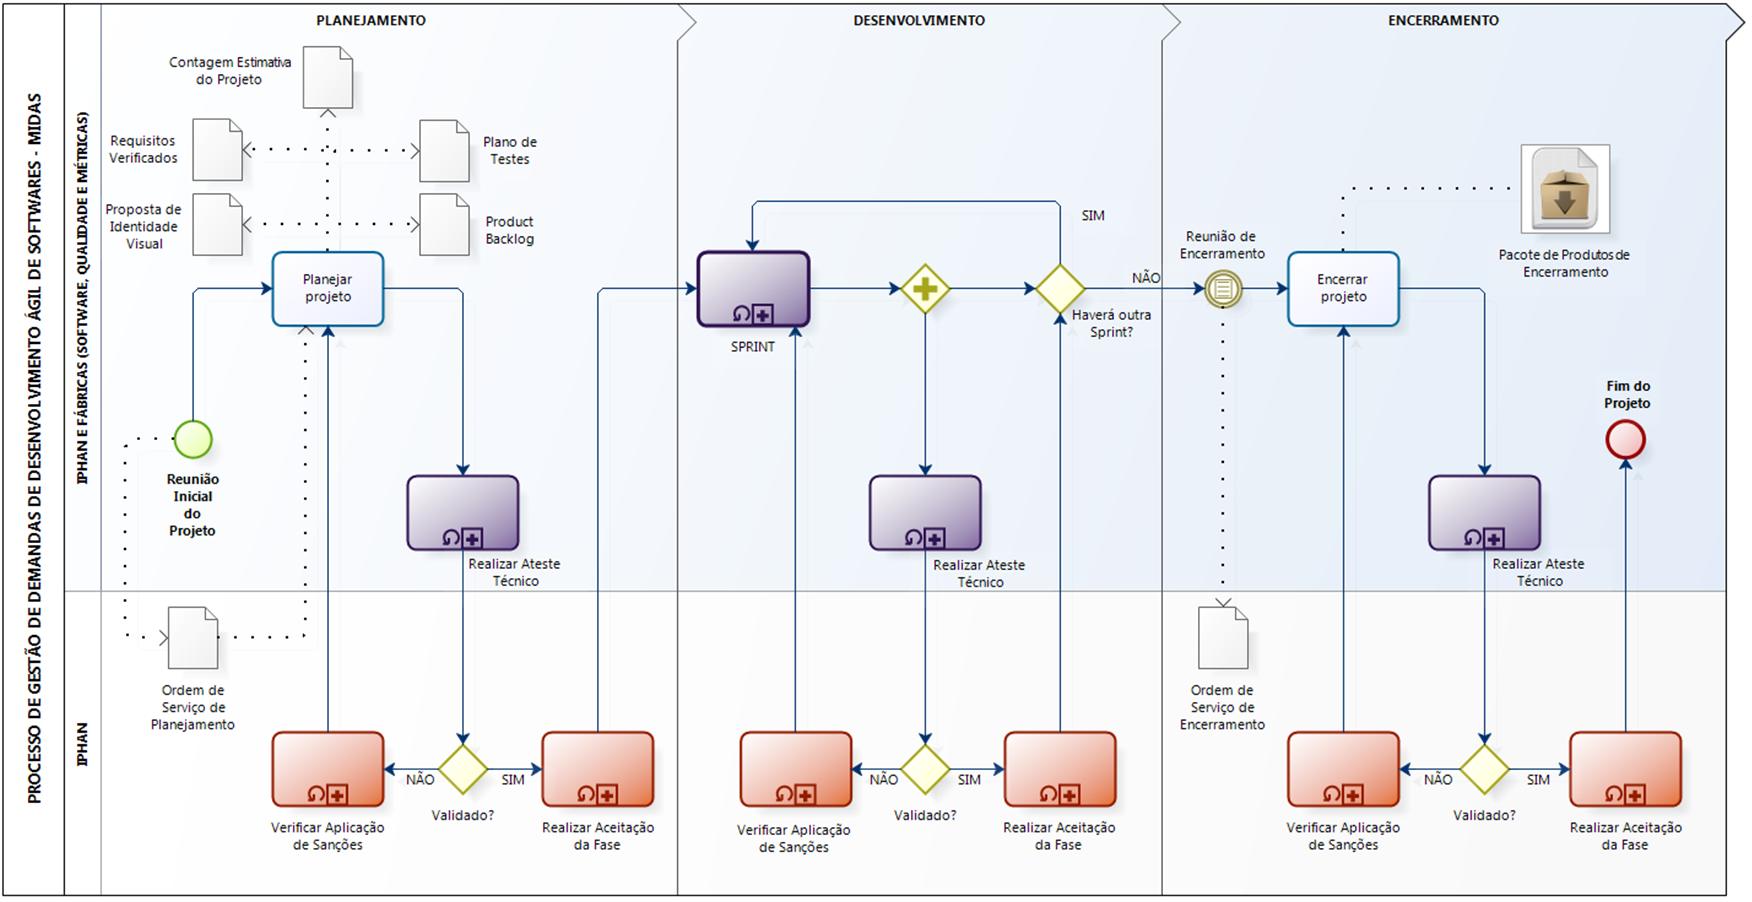
\includegraphics[scale=0.3]{figuras/processoMIDAS.png}
		\caption{Processo MIDAS \cite{IPHAN:2013}}
\end{figure}

O primeiro subprocesso advindo do planejamento é o subprocesso Realizar Ateste Técnico, trata-se de um subprocesso padrão que será executado em todas as fases do processo MIDAS. Nele estão contidos outros dois processos: Medição de Sistemas e Controle de Qualidade, cujo detalhamento não cabe no escopo deste trabalho. O subprocesso de Realizar Ateste Técnico tem o objetivo de verificar se os requisitos de cada fase foram satisfeitos e se os produtos de trabalho atendem às especificações de entrada e aos planos e regras estabelecidos. O fluxo deste subprocesso está representado na figura 22 com suas atividades, entradas e saídas.

\begin{figure}[h]
		\centering
		\label{fig01}
			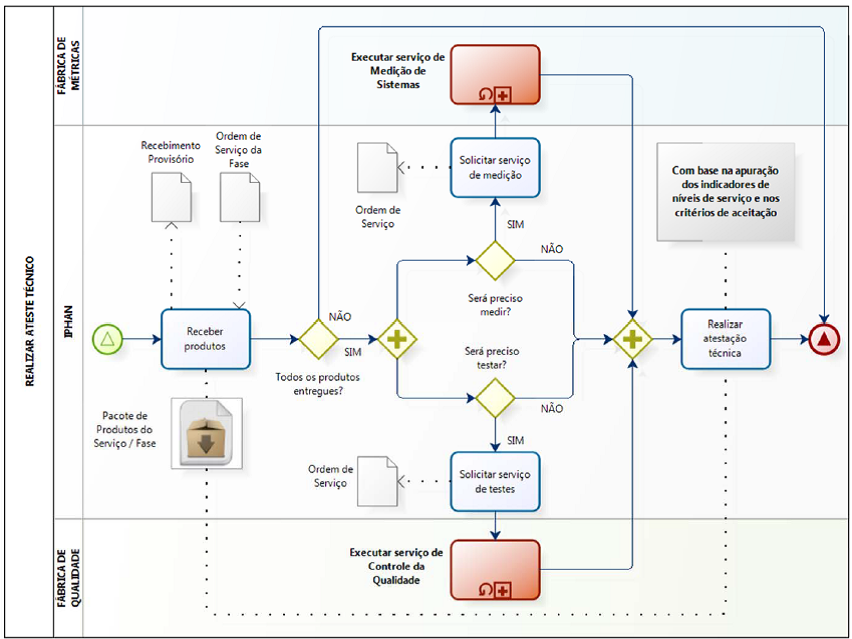
\includegraphics[scale=0.7]{figuras/subprocessoAteste.png}
		\caption{Subprocesso Realizar Ateste Técnico \cite{IPHAN:2013}}
\end{figure}

O subprocesso Sprint é o principal processo da fase de desenvolvimento e tem o objetivo de realizar o ciclo de trabalho de desenvolvimento. Sprint é um ciclo de desenvolvimento onde requisitos são implementados tendo como resultado um incremento do produto que está sendo desenvolvido. A quantidade de ciclos totais do projeto é definida na atividade de “Planejar Projeto”, a qual é realizada na fase de planejamento. O fluxo deste subprocesso está ilustrado na figura 23.


\begin{figure}[h]
		\centering
		\label{fig01}
			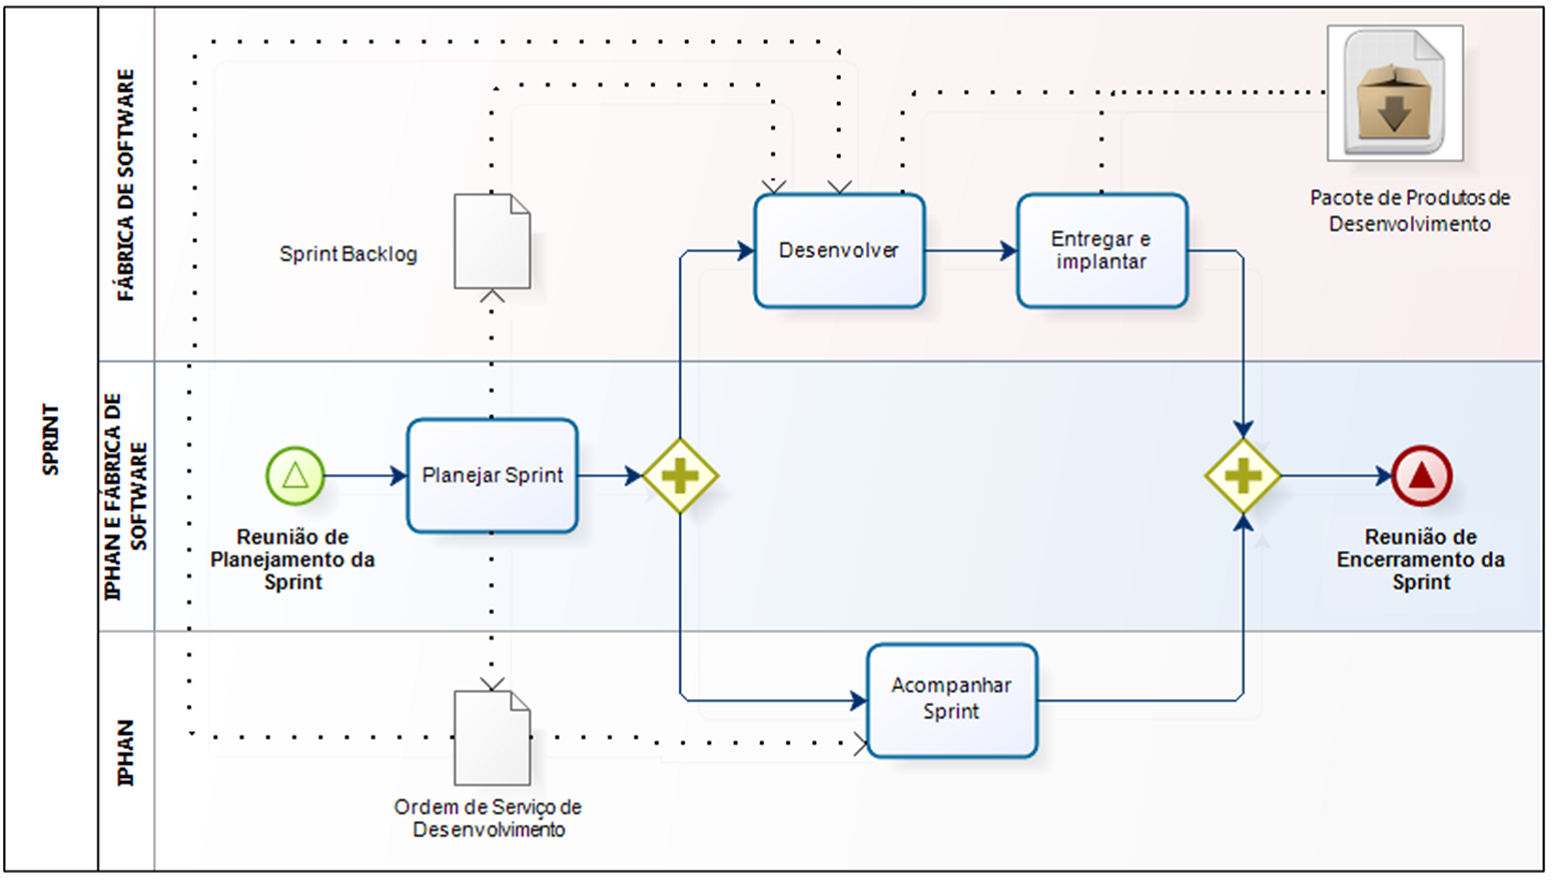
\includegraphics[scale=0.4]{figuras/subprocessoSprint.png}
		\caption{Subprocesso Sprint \cite{IPHAN:2013}}
\end{figure}

\end{anexosenv}

